%%%%%%%%%%%%%%%%%%%%%%%%%%%%%%%%%%%%%%%%%
% Homework Assignment Article
% LaTeX Template
% Version 1.3.1 (ECL) (08/08/17)
%
% This template has been downloaded from:
% Overleaf
%
% Original author:
% Victor Zimmermann (zimmermann@cl.uni-heidelberg.de)
%
% License:
% CC BY-SA 4.0 (https://creativecommons.org/licenses/by-sa/4.0/)
%
%%%%%%%%%%%%%%%%%%%%%%%%%%%%%%%%%%%%%%%%%

%----------------------------------------------------------------------------------------

\documentclass[a4paper]{article} % Uses article class in A4 format

%----------------------------------------------------------------------------------------
%	FORMATTING
%----------------------------------------------------------------------------------------

\addtolength{\hoffset}{-2.25cm}
\addtolength{\textwidth}{4.5cm}
\addtolength{\voffset}{-3.25cm}
\addtolength{\textheight}{5cm}
\setlength{\parskip}{0pt}
\setlength{\parindent}{0in}

%----------------------------------------------------------------------------------------
%	PACKAGES AND OTHER DOCUMENT CONFIGURATIONS
%----------------------------------------------------------------------------------------

\usepackage{blindtext} % Package to generate dummy text
% \usepackage[style=numeric,sorting=none]{biblatex}
\usepackage{charter} % Use the Charter font
\usepackage[utf8]{inputenc} % Use UTF-8 encoding
\usepackage{microtype} % Slightly tweak font spacing for aesthetics

\usepackage[english]{babel} % Language hyphenation and typographical rules

\usepackage{amsthm, amsmath, amssymb} % Mathematical typesetting
\usepackage{float} % Improved interface for floating objects
\usepackage[final, colorlinks = true, 
            linkcolor = black, 
            citecolor = black]{hyperref} % For hyperlinks in the PDF
\usepackage{graphicx, multicol} % Enhanced support for graphics
\usepackage{xcolor} % Driver-independent color extensions
\usepackage{marvosym, wasysym} % More symbols
\usepackage{rotating} % Rotation tools
\usepackage{censor} % Facilities for controlling restricted text
\usepackage{listings, style/lstlisting} % Environment for non-formatted code, !uses style file!
\usepackage{pseudocode} % Environment for specifying algorithms in a natural way
\usepackage{style/avm} % Environment for f-structures, !uses style file!
\usepackage{booktabs} % Enhances quality of tables

\usepackage{tikz-qtree} % Easy tree drawing tool
\tikzset{every tree node/.style={align=center,anchor=north},
         level distance=2cm} % Configuration for q-trees
\usepackage{style/btree} % Configuration for b-trees and b+-trees, !uses style file!

% \usepackage[backend=biber,style=numeric,
            % sorting=nyt]{biblatex} % Complete reimplementation of bibliographic facilities
% \addbibresource{ecl.bib}
\usepackage{csquotes} % Context sensitive quotation facilities

\usepackage[yyyymmdd]{datetime} % Uses YEAR-MONTH-DAY format for dates
\renewcommand{\dateseparator}{-} % Sets dateseparator to '-'

\usepackage{fancyhdr} % Headers and footers
\pagestyle{fancy} % All pages have headers and footers
\fancyhead{}\renewcommand{\headrulewidth}{0pt} % Blank out the default header
\fancyfoot[L]{School of Computing, Macquarie University} % Custom footer text
\fancyfoot[C]{} % Custom footer text
\fancyfoot[R]{\thepage} % Custom footer text

\usepackage{comment}
\newcommand{\note}[1]{\marginpar{\scriptsize \textcolor{red}{#1}}} % Enables comments in red on margin

%----------------------------------------------------------------------------------------

\begin{document}

%----------------------------------------------------------------------------------------
%	TITLE SECTION
%----------------------------------------------------------------------------------------

\title{COMP3100 project report} % Article title
\fancyhead[C]{}
\hrule \medskip % Upper rule
\begin{minipage}{1\textwidth} % Center of title section
\centering 
\large % Title text size
Project report: Stage 2\\ % Assignment title and number
COMP3100 Distributed Systems, S2, 2022\\
\normalsize % Subtitle text size
SID: 46030190, Name: Thien Luu \cite{code}
%%%%\\ % Assignment subtitle
\end{minipage}
\medskip\hrule % Lower rule
\bigskip

%----------------------------------------------------------------------------------------
%	ARTICLE CONTENTS
%----------------------------------------------------------------------------------------

%----------------------------------------------------------------------------------------
%	1 - INTRODUCTION (1/2 PAGE)
%----------------------------------------------------------------------------------------

\section{Introduction}
COMP3100 Stage 2 is continuing from Stage 1 where we built the foundation of communicating with a Distributed System and how to schedule jobs. Stage 2 of the assignment partly focuses on studying different scheduling algorithms, understanding them i.e. ‘First Fit’, ‘Best Fit’, ‘Worst Fit’, and ‘First Compatible’ and creating our own algorithm and implementing it.
\bigskip

The fore mentioned algorithms will be used as a baseline test and comparison with at least one of our own scheduling algorithm we develop. This scheduling algorithm we develop, we implement into our distributed system simulator, the main goal of this assignment being to optimise the average turnaround time and to NOT sacrifice any other performance metrics.
\bigskip

Like stage 1, we’ll have to write a report using \LaTeX, have evidence of project management, and demonstrate our written code with the chosen implemented algorithm.
Our goal of the project is to demonstrate our understanding of existing algorithms through report writing and research, and to develop our own algorithm to optimise average turnaround time through coding.

%----------------------------------------------------------------------------------------
%	2 - PROBLEM OVERVIEW (1/2 PAGE)
%----------------------------------------------------------------------------------------

\section{Problem Overview}
\label{sec:section2}
There are existing scheduling algorithms such as aforementioned, first fit, best fit, worst fit, and first compatible that are suitable and most efficient for certain cases. However in our distributed system the goal is to achieve a better turnaround time and these existing algorithms are limited. Another problem is we can’t sacrifice other performance metrics to achieving a better average turnaround time.
\bigskip

Taking into consideration, the Distributed System Simulator may have jobs to be scheduled, each job having different requirements. Potentially a job that is scheduled may be using unnecessary resources, and the next jobs to be scheduled and allocated to this server will have to wait resulting in a long turnaround time.
\bigskip

This can be resolved by using more readily available resources outside what’s been initially provided to only work with, however we sacrifice other performance metrics resulting in higher costs.


%----------------------------------------------------------------------------------------
%	3 - ALGORITHM DESCRIPTION (1 PAGE)
%----------------------------------------------------------------------------------------
\break
\section{Algorithm Description}
\label{sec:section3}
The scheduling algorithm adopts a feature of the worst fit algorithm where it selects the largest server that is ‘available’ first, and schedules a job to it which then all it's resources are occupied. The next job is scheduled on the biggest server 'available' and so fourth.
\medskip

This modified version of the worst fit algorithm, upon scheduling, a job is scheduled on the largest server ‘available’. If there is remaining resources for this server, and meets the requirements of the next job to be scheduled, this job will be scheduled on this server. If not, then it’ll be scheduled onto the next largest ‘available’ server. This process will repeat until a job is completed.
\medskip

When a job is completed, the resource is free’d. Depending on the requirements of the next job, if there’s enough resource, the job is then scheduled. If all servers are busy running with no remaining resources to support the next job, then it’ll be queued.

\medskip
The queue is determined by selecting the server with the least amount of queued jobs. This repeats, evenly distributing, queuing jobs across the servers.

\subsection*{Sample Scheduling Scenario}
Below there are 2 servers, one small with 2 cores, and one medium with 4 cores. There are 5 jobs, 2 with 1 cores, 2 with 2 cores and 1 with 4 cores. They are scheduled regardless of memory or disk usage. In teh scheduling algorithm the memory and disk usage is considered to get the available servers.

\begin{figure}[!h]
    \centering
    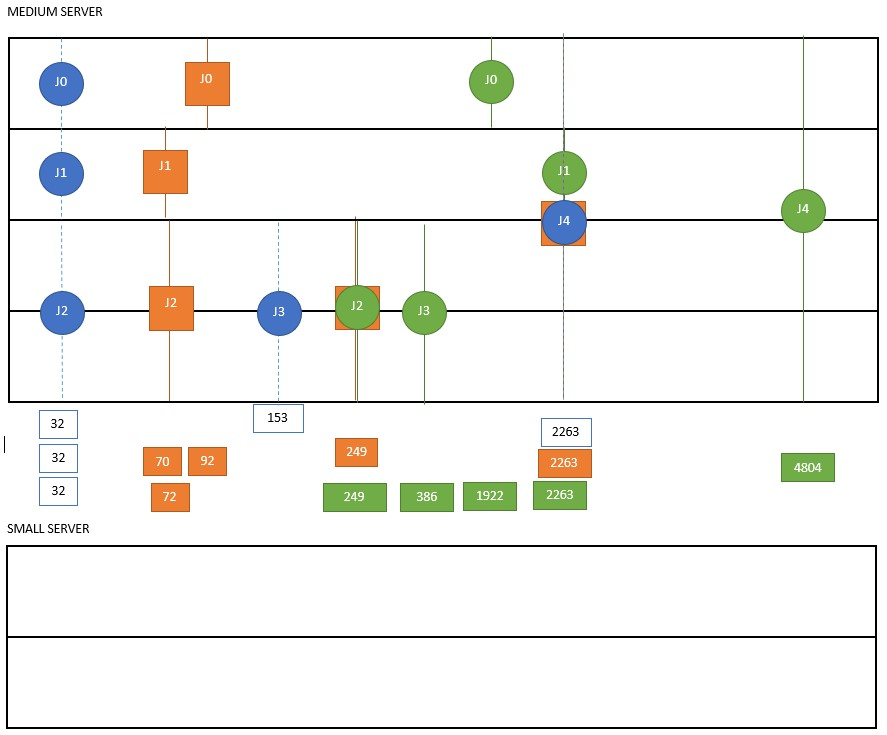
\includegraphics[width=17cm]{images/MySchedulingDiagram.jpg}
    \caption{My Scheduling Algorithm Diagram}
    \label{fig:my_label}
\end{figure}

%----------------------------------------------------------------------------------------
%	4 - IMPLEMENTATION (1/2 PAGE)
%----------------------------------------------------------------------------------------
\break
\section{Implementation}
\subsection*{Classes}
\textbf{-=Server=- \textit{implements} Comparable}
\begin{flushleft}
    \begin{tabular}{|l|l|l|}
        \hline
        \textbf{Attribute Name} & \textbf{Data Type} & \textbf{Description} \\
        \hline
        Type & String & Type of Server \\
        \hline
        ServerId & Integer & Identification number of Server\\
        \hline
        ServerState & String & State of Server\\
        \hline
        CurStartTime & Integer & Start time of Server\\
        \hline
        Cores & Integer & Number of cores on Server\\
        \hline
        Memory & Integer & Size of memory for Server\\
        \hline
        Disk & Integer & Disk space for Server\\
        \hline
        wJobs & Integer & Number of jobs waiting\\
        \hline
        rJobs & Integer & Number of jobs running\\
        \hline
        estTime & Integer & Sum of estimated runtime of jobs queued and running\\
        \hline
    \end{tabular}
\end{flushleft}

\textbf{-=Job=-}
\begin{flushleft}
    \begin{tabular}{|l|l|l|}
        \hline
        \textbf{Attribute Name} & \textbf{Data Type} & \textbf{Description} \\
        \hline
        submitTime & Integer & Submission time to server\\
        \hline
        jobId & Integer & Identification number of Job\\
        \hline
        estRuntime & Integer & Estimated runtime\\
        \hline
        core & Integer & Required cores\\
        \hline
        Memory & Integer & Required memory\\
        \hline
        Disk & Integer & Required disk space\\
        \hline
        jobState & Integer & State of job - Running or waiting\\
        \hline
    \end{tabular}
\end{flushleft}

The idea behind implementing the scheduling algorithm requires the commands:

\begin{enumerate}
    \item GETS Available
    \item GETS Capable
\end{enumerate}

Primarily the 'GETS Available' command is used to achieve the scheduling algorithm, it gives back a list of immediately available servers for a job. The list is already sorted from smallest to largest by type. The largest server being at the bottom of the list is used first and then this process repeats, requests available servers, and schedules jobs to the largest server at the bottom of the list.
\medskip

But when there are no immediately available servers when the command is called, the 'GETS Capable' is then used to assist. This command gets a list of all servers capable of running the next scheduled job. This list of servers will then be sorted based on how many jobs they have. The server capable of running the job, with the least amount of jobs will then be queued with the next job. This process evenly distributes, queuing the jobs across the servers.

\subsection*{Not Implemented}
An attempt was made to improve the efficiency of the algorithm by using the 'MIGJ' command. Where when a job is completed, a search is conducted across all servers. The server with the largest amount of queued jobs, a job from this server, an attempt is made to migrate it to a server that is 'idle' or 'inactive'. This attempt evenly distributes jobs that are in a long queue, and placed on an 'available' server to immediately run. The attempt can be seen in the branch 2.1.

%----------------------------------------------------------------------------------------
%	5 - EVALUATION (2 PAGE)
%----------------------------------------------------------------------------------------
\break
\section{Evaluation}
The Stage2-test suite was used with the new algorithm to acquire these \textbf{average results}. This test suite contained 18 configurations.

\begin{figure}[!h]
    \centering
    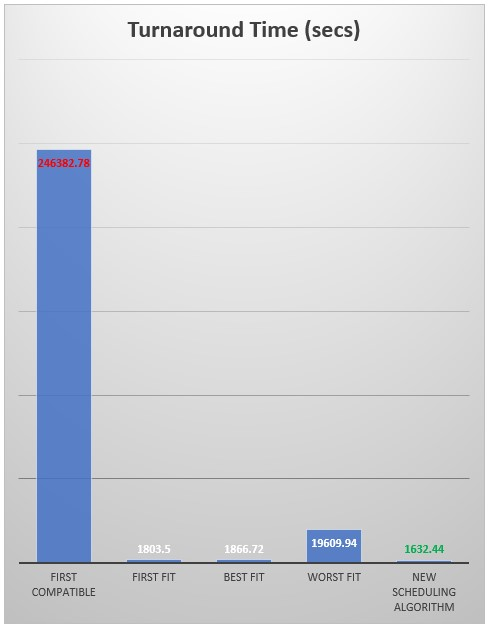
\includegraphics[width=8.5cm]{images/TurnaroundTimeDiagram.jpg}
    \label{fig:my_label}
\end{figure}
In terms of turnaround time, the new algorithm performed overall on average better than existing algorithms. The worst performing algorithm was the 'First Compatible', performing roughly 150x worst than the new algorithm.
\medskip

The results provided by the test suite showed 6 of 18 configurations where our algorithm performed better than all the existing algorithms. The ones that didn't, only performed better for Worst Fit and First Capable. Our algorithm requires some features of First Fit and Best Fit to further improve the turnaround time. It seems with Best Fit, the search for the correct fitment of jobs to be scheduled on the server allows for the improve efficiency which the new algorithm does not currently have.

\begin{figure}
\centering
    \begin{minipage}{.5\textwidth}
      \centering
        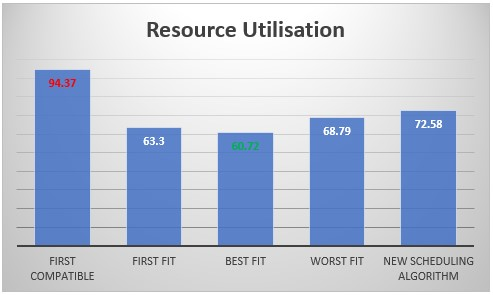
\includegraphics[width=7cm]{images/ResourceUtilizationDiagram.jpg}
      \label{fig:test1}
    \end{minipage}%
    \begin{minipage}{.5\textwidth}
      \centering
        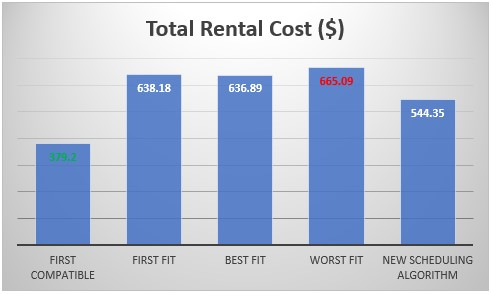
\includegraphics[width=7cm]{images/TotalRentalCostDiagram.jpg}
      \label{fig:test2}
    \end{minipage}
    \begin{flushleft}
        Resource Utilisation, our new algorithm did perform better in most cases better than some algorithms. Only one of the cases of the 18 was worst. Overall the average of the new algorithm was only better than the First Capable.
        \medskip
        
        Total Rental Cost, our new algorithm did perform better in most cases better than some algorithms. Overall the average of the new algorithm was better than all existing algorithms but First Capable.
    \end{flushleft}
\end{figure}

%----------------------------------------------------------------------------------------
%	6 - CONCLUSION (1/4 PAGE)
%----------------------------------------------------------------------------------------
\break
\section{Conclusion}
In conclusion, the new scheduling algorithm can be further improved with features of other scheduling algorithms through calculations it wasn't able to outperform. But overall the turnaround time average was better. There was some sacrificing of performance metrics when compared to some of the existing scheduling algorithms, so in conclusion this is average.

%----------------------------------------------------------------------------------------
%	7 - REFERENCE LIST
%----------------------------------------------------------------------------------------

\bibliographystyle{ieeetr}
\bibliography{comp3100project}
% \printbibliography

%----------------------------------------------------------------------------------------

\end{document}